\begin{reviewed}

    \subsection*{Quantitative Overview of the Field}\label{subsec:results_quantitative}
    % -----------------------------------------------------------------------

    The distribution of the selected literature across the seven concept-matrix categories is illustrated in Figure~\ref{fig:distribution_topics}. As described in Section~\ref{sec:severity_scoring_methodology}, each category was independently scored on four severity dimensions by five domain-expert raters, so that this literature coverage can be compared against assessed severity rather than treated as a proxy for it.

    \begin{table}[h]
        \centering
        \small
        \caption{Mean severity dimension scores across 5 raters. The final row presents ordinal Krippendorff's $\alpha$ to measure inter-rater reliability for each dimension: Magnitude (M), Certainty (C), Irreversibility (I) and Scope (S). The \textit{Severity} column is the unweighted mean of the four dimension means and is the input to Table~\ref{tab:severity_coverage}.}
        \label{tab:rater_scores_summary}
        \begin{tabular}{|l|c|c|c|c|c|}
            \hline
            \textbf{Category} & \textbf{M} & \textbf{C} & \textbf{I} & \textbf{S} & \textbf{Severity} \\
            \hline
            Human \& Societal Impacts         & 4.2 & 3.8 & 3.8 & 4.6 & \textbf{4.10} \\
            Governance, Regulation \& Policy  & 4.2 & 3.6 & 3.8 & 4.0 & 3.90 \\
            Alignment                         & 4.2 & 3.6 & 3.6 & 3.4 & 3.70 \\
            Auditing, Safety \& Oversight     & 3.6 & 4.2 & 3.4 & 3.0 & 3.55 \\
            Bias \& Fairness                  & 3.0 & 4.0 & 3.2 & 3.4 & 3.40 \\
            Liability \& Ethics               & 3.8 & 3.4 & 2.2 & 2.8 & 3.05 \\
            Explainability / Interpretability & 3.0 & 3.4 & 2.4 & 3.4 & 3.05 \\
            \hline \hline
            \textit{Krippendorff's $\alpha$}  & 0.027 & $-0.113$ & 0.048 & 0.122 & --- \\
            \hline
        \end{tabular}
    \end{table}

    Inter-rater reliability (IRR) was evaluated by calculating ordinal Krippendorff's $\alpha$ for each severity dimension across the seven categories. As presented in the final row of Table~\ref{tab:rater_scores_summary}, agreement across all four dimensions was near zero, well below the standard $\sim$0.67 threshold for acceptable agreement. Given this lack of consensus, and the low number of raters ($n=5$), the severity scores that follow should be treated as indicative rather than definitive; they summarize the raters' central tendency but do not reflect a shared understanding of relative risk across the seven categories.

    \subsubsection{Severity and Coverage}

\begin{toreview}

    Table~\ref{tab:severity_coverage} compares severity scores with the number of category assignments. The review contains 80 distinct included entries: 63 from the systematic search and 17 introduced through snowballing. Because each entry could be assigned to more than one category, these entries produced 135 category assignments in total.

\end{toreview}

	\begin{reviewed}

	\begin{table}[h]
	\centering
	\scriptsize
	\caption{Category coverage against a severity-weighted expectation. The 80 distinct included entries produced 135 category assignments because entries could be assigned to multiple categories. Each severity point corresponds to $135/24.75=5.45$ assignments, so Expected is the category's severity multiplied by that rate. Actual $-$ Exp.\ is Assignments minus Expected; Coverage is Assignments divided by Expected, where $1.00$ means the category has exactly the coverage its severity predicts.}
	\label{tab:severity_coverage}
	\resizebox{\textwidth}{!}{%
	\begin{tabular}{lrrrrr}
	\toprule
	Category & Severity & Assignments & Expected & Actual $-$ Exp. & Coverage \\
	\midrule
	Human \& Societal Impacts    & 4.10 & 32 & 22.4 & $+9.6$ & 1.43 \\
	Governance, Reg.\ \& Policy   & 3.90 & 25 & 21.3 & $+3.7$ & 1.18 \\
	Alignment                     & 3.70 & 30 & 20.2 & $+9.8$ & 1.49 \\
	Auditing, Safety \& Oversight & 3.55 & 19 & 19.4 & $-0.4$ & 0.98 \\
	Bias \& Fairness              & 3.40 & 9  & 18.5 & $-9.5$ & 0.49 \\
	Liability \& Ethics           & 3.05 & 8  & 16.6 & $-8.6$ & 0.48 \\
	Explainability / Interp.      & 3.05 & 12 & 16.6 & $-4.6$ & 0.72 \\
	\bottomrule
	\end{tabular}
	}
	\end{table}

	Severity and coverage do not align perfectly. \emph{Bias \& Fairness} is the clearest case: it scores higher in severity (3.40) than either \emph{Explainability / Interpretability} or \emph{Liability \& Ethics} (both 3.05), yet has fewer assignments (9) than Explainability (12) and only one more than Liability (8). All three fall below what their severity predicts, with coverage ratios of 0.49, 0.48, and 0.72 respectively. At the other end, \emph{Governance, Regulation \& Policy} ranks second in severity but has fewer assignments than \emph{Alignment}, though both exceed their expected counts. \emph{Auditing, Safety \& Oversight} lands almost exactly on its expectation. Overall, research attention broadly follows assessed severity, but some categories receive relatively more or less attention than their severity would suggest.
		
	\end{reviewed}

    % To keep this I would need a citation
    % The relationship between severity and literature coverage can be assessed using Spearman's rank correlation. Using the severity and coverage ranks, the squared rank differences sum to $\sum d_i^2 = 6$. With seven categories, this gives
    % \[
    % \rho = 1 - \frac{6\sum d_i^2}{n(n^2-1)}
    %     = 1 - \frac{6(6)}{7(7^2-1)}
    %     = 0.893.
    % \]
    % This indicates a strong positive association between severity and research coverage: categories ranked as more severe generally receive more research attention. Given the small number of categories ($n=7$), this result should be interpreted cautiously.

	\begin{figure}[htbp]
		\centering
		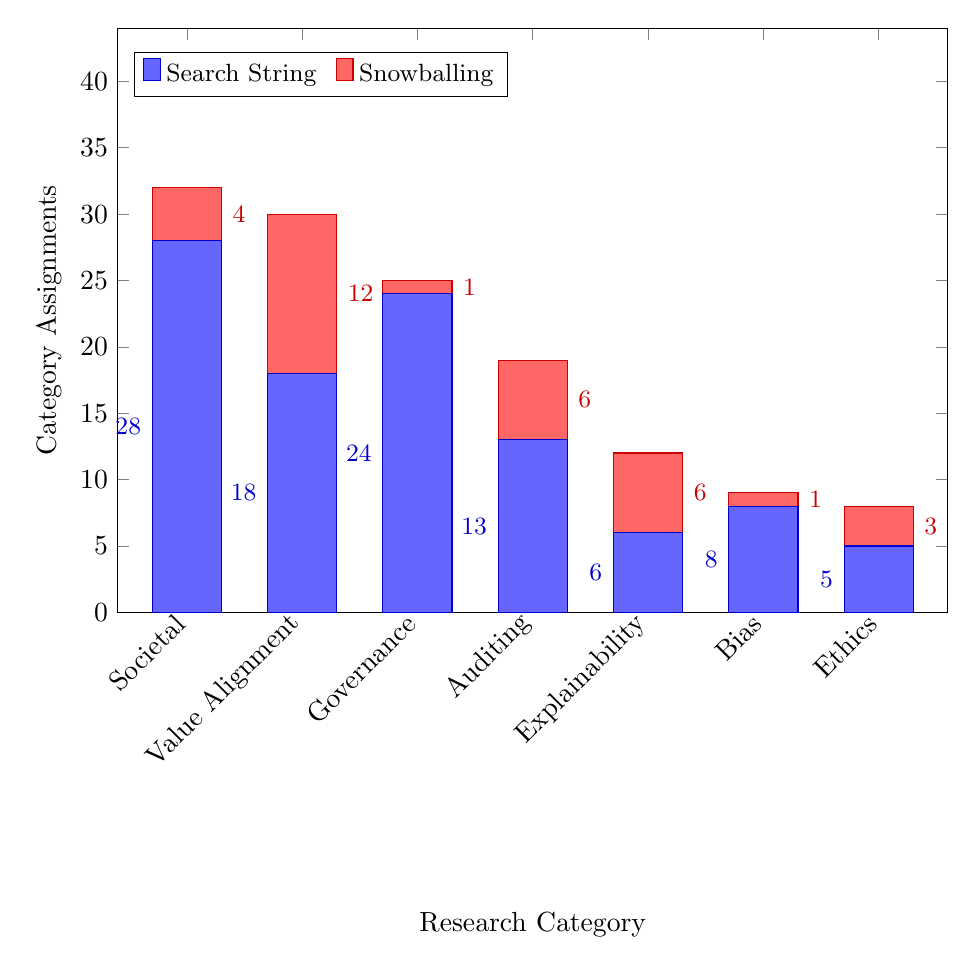
\begin{tikzpicture}
		\begin{axis}[
			ybar stacked,
			symbolic x coords={Societal, Value Alignment, Governance, Auditing, Explainability, Bias, Ethics},
			xtick=data,
			x tick label style={rotate=45, anchor=east},
			ylabel={Category Assignments},
			xlabel={Research Category},
			xlabel style={yshift=-1.5cm},
			width=\textwidth,
			height=9cm,
			bar width=25pt,
			ymin=0,
			ymax=44,
			legend style={
				at={(0.02,0.96)},
				anchor=north west,
				legend columns=-1,
				font=\small,
				/tikz/every even column/.append style={column sep=5pt}
			}
		]

		% Plot 1: Search String (bottom, BLUE)
		\addplot [
			fill=blue!60,
			draw=blue!80!black,
			nodes near coords,
			every node near coord/.style={
				color=blue!80!black,
				font=\small,
				anchor=east,
				xshift=-13pt,
			},
		] coordinates {
			(Societal,28) (Value Alignment,18) (Governance,24)
			(Auditing,13) (Explainability,6) (Bias,8) (Ethics,5)
		};

		% Plot 2: Snowballing (top, RED)
		\addplot [
			fill=red!60,
			draw=red!80!black,
			nodes near coords,
			every node near coord/.style={
				color=red!80!black,
				font=\small,
				anchor=west,
				xshift=13pt,
			},
			point meta=explicit symbolic,
		] coordinates {
			(Societal,4)       [4]
			(Value Alignment,12)     [12]
			(Governance,1)     [1]
			(Auditing,6)       [6]
			(Explainability,6) [6]
			(Bias,1)           [1]
			(Ethics,3)         [3]
		};

		% Plot 3: Invisible - bold black totals above each bar
		\addplot [
			draw=none, fill=none,
			forget plot,
			nodes near coords,
			every node near coord/.style={
				anchor=south,
				yshift=3pt,
				font=\small\bfseries,
				color=black,
			},
			point meta=explicit symbolic,
		] coordinates {
			(Societal,0)       [32]
			(Value Alignment,0)      [30]
			(Governance,0)     [25]
			(Auditing,0)       [19]
			(Explainability,0) [12]
			(Bias,0)           [9]
			(Ethics,0)         [8]
		};

		\legend{Search String, Snowballing}
		\end{axis}
		\end{tikzpicture}
		\caption{Distribution of category assignments across the 80 included entries. Entries assigned to multiple categories are counted once in each applicable category.}
		\label{fig:distribution_topics}
	\end{figure}

    \vspace{1.5em}

\end{reviewed}
